\part{Recursion}
\frame{\partpage}

\begin{frame}[fragile]{Recursion}
    \begin{itemize}
        \pause\item A \textbf{recursive} function is a function that \textbf{calls itself}
        \pause\item Example: the \textbf{Fibonacci numbers} --- each number in the sequence is the sum of the previous two
    $$ 1, 1, 2, 3, 5, 8, 13, 21, 34, 55, \dots $$
        \pause\item To calculate the $n$th Fibonacci number:
    \end{itemize}
    \begin{lstlisting}
int fibonacci(int n)
{
    if (n <= 2)
        return 1;
    else
        return fibonacci(n-1) + fibonacci(n-2);
}
    \end{lstlisting}
    \begin{itemize}
        \pause\item Recursive functions need a \textbf{base case} where they stop recursing,
			otherwise they will go \textbf{forever}
    \end{itemize}
\end{frame}

\begin{frame}{Thinking recursively}
	\begin{itemize}
		\pause\item I want to solve a problem
		\pause\item If I already had a function to solve smaller instances of the problem, I could use it
			to write my function
		\pause\item I can solve the smallest possible problem
		\pause\item Therefore I can write a recursive function
	\end{itemize}
\end{frame}

\begin{frame}{Example: file sizes}
    \begin{itemize}
        \pause\item Suppose we want to find the total size of all files in a folder and its subfolders
    \end{itemize}
    \pause
    \begin{center}
        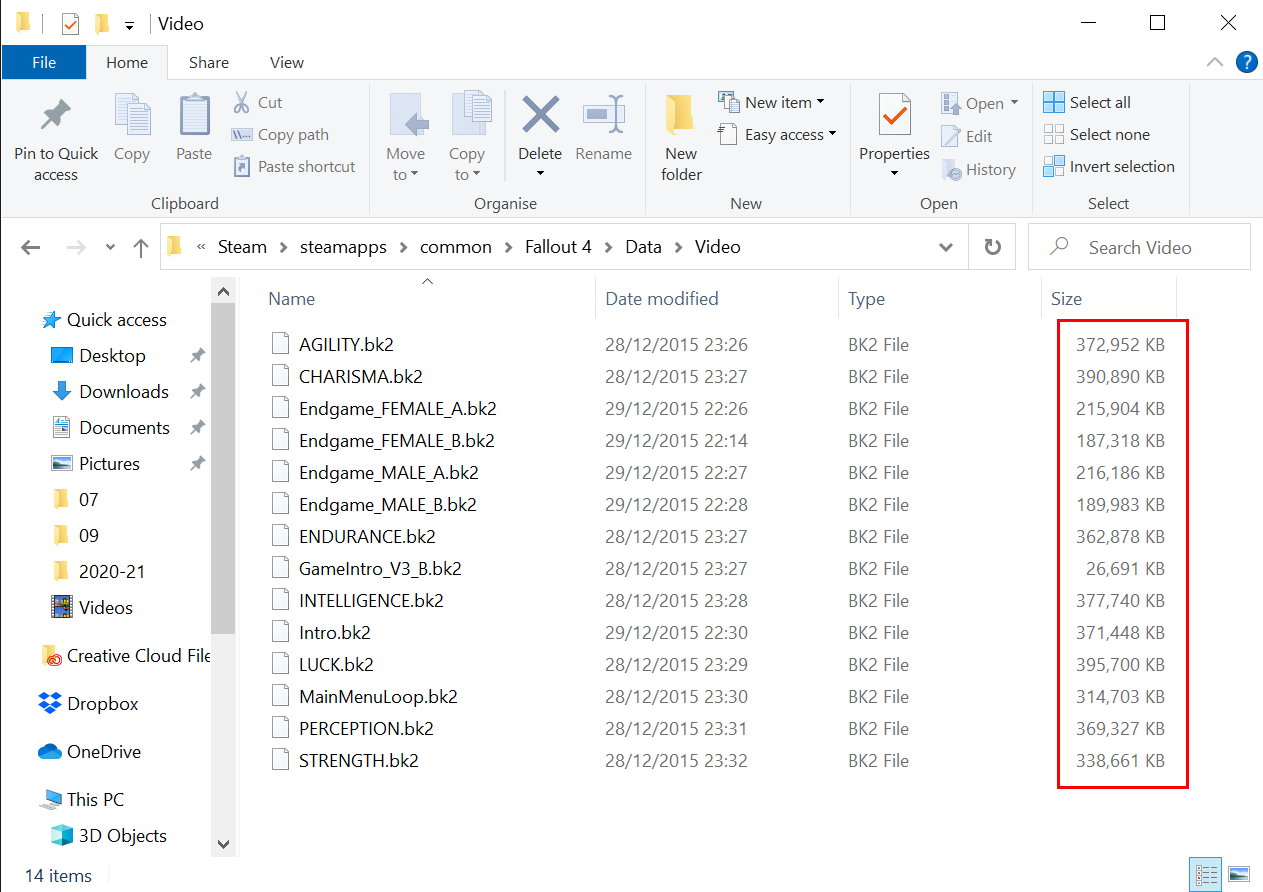
\includegraphics[height=0.5\textheight]{filesizes_1}
    \end{center}
    \begin{itemize}
        \item If the folder contains \textbf{only} files, then we can simply add their sizes together
    \end{itemize}
\end{frame}

\begin{frame}{Example: file sizes}
    \begin{itemize}
        \item What if the folder contains subfolders?
    \end{itemize}
    \begin{center}
        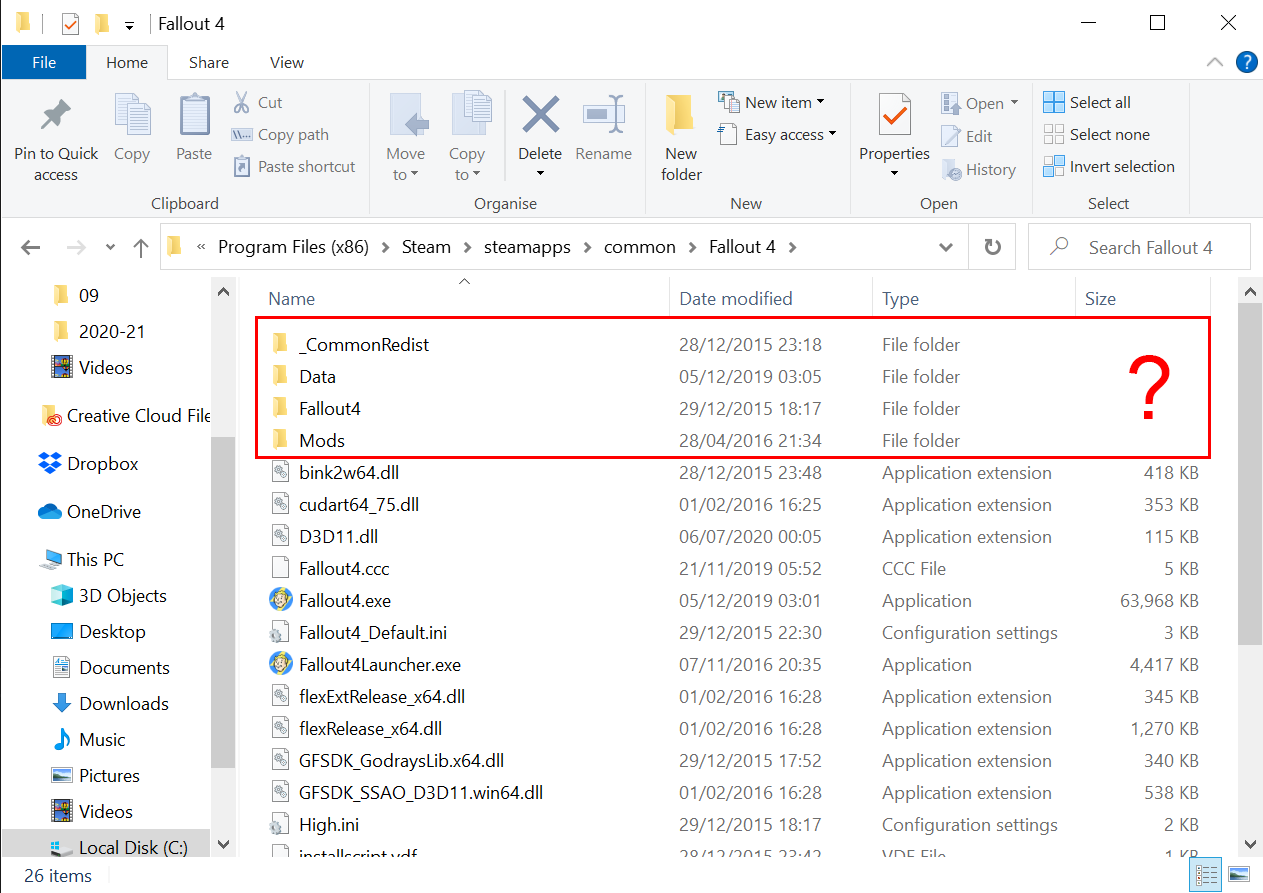
\includegraphics[height=0.5\textheight]{filesizes_2}
    \end{center}
    \begin{itemize}
        \pause\item We need to find the total size of all files in the subfolders and their subsubfolders...
    \end{itemize}
\end{frame}

\begin{frame}{Example: file sizes --- recursive solution}
    \footnotesize
    \begin{algorithmic}
        \State assume the system provides a \Call{GetFileSize}{} function \pause
        \Procedure{CalculateFolderSize}{$folder$} \pause
            \State $totalSize \gets 0$ \pause
            \For {each $item$ in $folder$} \pause
                \If {$item$ is a file}
                    \State $totalSize \gets totalSize + \Call{GetFileSize}{item}$ \pause
                \ElsIf {$item$ is a folder}
                    \State $totalSize \gets totalSize + \Call{CalculateFolderSize}{item}$ \pause
                \EndIf
            \EndFor
            \State \textbf{return} totalSize \pause
        \EndProcedure
    \end{algorithmic}
\end{frame}

\begin{frame}{The call stack}
	\begin{itemize}
        \pause\item Recall: nested function calls are handled using a \textbf{stack}
        \pause\item \textbf{Calling} a function \textbf{pushes} a frame onto the stack
        \pause\item \textbf{Returning} from a function \textbf{pops} the top frame from the stack
		\pause\item Recursive functions are no different
		\pause\item This means if a recursive function contains \textbf{local variables},
            they are \textbf{independent} between instances of the function
        \pause\item This is also why careless use of recursion can lead to a \textbf{stack overflow}
	\end{itemize}
\end{frame}
